% Created by tikzDevice version 0.12 on 2020-05-12 17:36:37
% !TEX encoding = UTF-8 Unicode
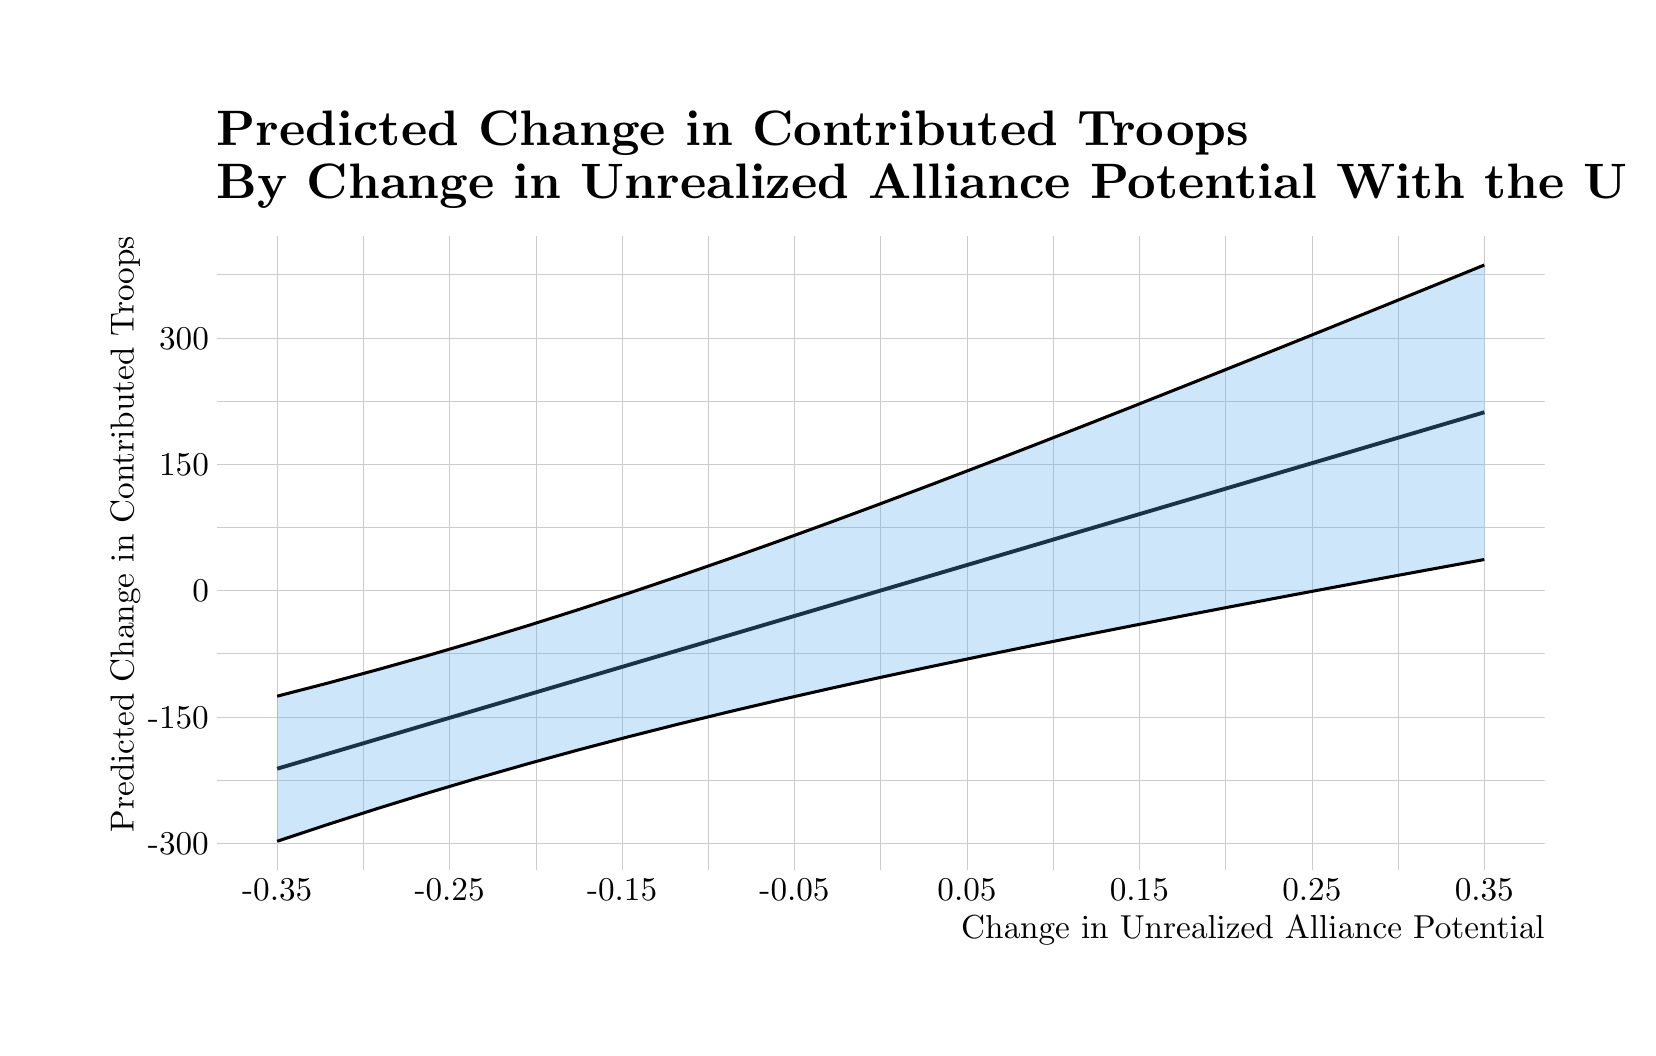
\begin{tikzpicture}[x=1pt,y=1pt]
\definecolor{fillColor}{RGB}{255,255,255}
\path[use as bounding box,fill=fillColor,fill opacity=0.00] (0,0) rectangle (578.16,361.35);
\begin{scope}
\path[clip] ( 68.34, 56.94) rectangle (548.16,285.99);
\definecolor{drawColor}{gray}{0.80}

\path[draw=drawColor,line width= 0.2pt,line join=round] ( 68.34, 89.49) --
	(548.16, 89.49);

\path[draw=drawColor,line width= 0.2pt,line join=round] ( 68.34,135.15) --
	(548.16,135.15);

\path[draw=drawColor,line width= 0.2pt,line join=round] ( 68.34,180.80) --
	(548.16,180.80);

\path[draw=drawColor,line width= 0.2pt,line join=round] ( 68.34,226.45) --
	(548.16,226.45);

\path[draw=drawColor,line width= 0.2pt,line join=round] ( 68.34,272.10) --
	(548.16,272.10);

\path[draw=drawColor,line width= 0.2pt,line join=round] (121.31, 56.94) --
	(121.31,285.99);

\path[draw=drawColor,line width= 0.2pt,line join=round] (183.62, 56.94) --
	(183.62,285.99);

\path[draw=drawColor,line width= 0.2pt,line join=round] (245.94, 56.94) --
	(245.94,285.99);

\path[draw=drawColor,line width= 0.2pt,line join=round] (308.25, 56.94) --
	(308.25,285.99);

\path[draw=drawColor,line width= 0.2pt,line join=round] (370.57, 56.94) --
	(370.57,285.99);

\path[draw=drawColor,line width= 0.2pt,line join=round] (432.88, 56.94) --
	(432.88,285.99);

\path[draw=drawColor,line width= 0.2pt,line join=round] (495.19, 56.94) --
	(495.19,285.99);

\path[draw=drawColor,line width= 0.2pt,line join=round] ( 68.34, 66.67) --
	(548.16, 66.67);

\path[draw=drawColor,line width= 0.2pt,line join=round] ( 68.34,112.32) --
	(548.16,112.32);

\path[draw=drawColor,line width= 0.2pt,line join=round] ( 68.34,157.97) --
	(548.16,157.97);

\path[draw=drawColor,line width= 0.2pt,line join=round] ( 68.34,203.62) --
	(548.16,203.62);

\path[draw=drawColor,line width= 0.2pt,line join=round] ( 68.34,249.27) --
	(548.16,249.27);

\path[draw=drawColor,line width= 0.2pt,line join=round] ( 90.15, 56.94) --
	( 90.15,285.99);

\path[draw=drawColor,line width= 0.2pt,line join=round] (152.47, 56.94) --
	(152.47,285.99);

\path[draw=drawColor,line width= 0.2pt,line join=round] (214.78, 56.94) --
	(214.78,285.99);

\path[draw=drawColor,line width= 0.2pt,line join=round] (277.09, 56.94) --
	(277.09,285.99);

\path[draw=drawColor,line width= 0.2pt,line join=round] (339.41, 56.94) --
	(339.41,285.99);

\path[draw=drawColor,line width= 0.2pt,line join=round] (401.72, 56.94) --
	(401.72,285.99);

\path[draw=drawColor,line width= 0.2pt,line join=round] (464.04, 56.94) --
	(464.04,285.99);

\path[draw=drawColor,line width= 0.2pt,line join=round] (526.35, 56.94) --
	(526.35,285.99);
\definecolor{drawColor}{RGB}{0,0,0}

\path[draw=drawColor,line width= 1.4pt,line join=round] ( 90.15, 93.57) --
	(108.33, 98.93) --
	(126.50,104.30) --
	(144.68,109.67) --
	(162.85,115.03) --
	(181.03,120.40) --
	(199.20,125.77) --
	(217.38,131.14) --
	(235.55,136.50) --
	(253.73,141.87) --
	(271.90,147.24) --
	(290.08,152.60) --
	(308.25,157.97) --
	(326.43,163.34) --
	(344.60,168.70) --
	(362.78,174.07) --
	(380.95,179.44) --
	(399.13,184.81) --
	(417.30,190.17) --
	(435.48,195.54) --
	(453.65,200.91) --
	(471.83,206.27) --
	(490.00,211.64) --
	(508.18,217.01) --
	(526.35,222.37);
\definecolor{fillColor}{RGB}{92,172,238}

\path[fill=fillColor,fill opacity=0.30] ( 90.15,119.78) --
	(108.33,124.48) --
	(126.50,129.38) --
	(144.68,134.49) --
	(162.85,139.82) --
	(181.03,145.36) --
	(199.20,151.12) --
	(217.38,157.07) --
	(235.55,163.22) --
	(253.73,169.53) --
	(271.90,176.01) --
	(290.08,182.62) --
	(308.25,189.35) --
	(326.43,196.19) --
	(344.60,203.13) --
	(362.78,210.14) --
	(380.95,217.23) --
	(399.13,224.38) --
	(417.30,231.58) --
	(435.48,238.82) --
	(453.65,246.11) --
	(471.83,253.43) --
	(490.00,260.79) --
	(508.18,268.17) --
	(526.35,275.58) --
	(526.35,169.17) --
	(508.18,165.84) --
	(490.00,162.49) --
	(471.83,159.11) --
	(453.65,155.70) --
	(435.48,152.26) --
	(417.30,148.77) --
	(399.13,145.24) --
	(380.95,141.65) --
	(362.78,138.00) --
	(344.60,134.28) --
	(326.43,130.48) --
	(308.25,126.59) --
	(290.08,122.59) --
	(271.90,118.47) --
	(253.73,114.21) --
	(235.55,109.79) --
	(217.38,105.20) --
	(199.20,100.42) --
	(181.03, 95.44) --
	(162.85, 90.25) --
	(144.68, 84.84) --
	(126.50, 79.22) --
	(108.33, 73.39) --
	( 90.15, 67.36) --
	cycle;

\path[] ( 90.15,119.78) --
	(108.33,124.48) --
	(126.50,129.38) --
	(144.68,134.49) --
	(162.85,139.82) --
	(181.03,145.36) --
	(199.20,151.12) --
	(217.38,157.07) --
	(235.55,163.22) --
	(253.73,169.53) --
	(271.90,176.01) --
	(290.08,182.62) --
	(308.25,189.35) --
	(326.43,196.19) --
	(344.60,203.13) --
	(362.78,210.14) --
	(380.95,217.23) --
	(399.13,224.38) --
	(417.30,231.58) --
	(435.48,238.82) --
	(453.65,246.11) --
	(471.83,253.43) --
	(490.00,260.79) --
	(508.18,268.17) --
	(526.35,275.58);

\path[] (526.35,169.17) --
	(508.18,165.84) --
	(490.00,162.49) --
	(471.83,159.11) --
	(453.65,155.70) --
	(435.48,152.26) --
	(417.30,148.77) --
	(399.13,145.24) --
	(380.95,141.65) --
	(362.78,138.00) --
	(344.60,134.28) --
	(326.43,130.48) --
	(308.25,126.59) --
	(290.08,122.59) --
	(271.90,118.47) --
	(253.73,114.21) --
	(235.55,109.79) --
	(217.38,105.20) --
	(199.20,100.42) --
	(181.03, 95.44) --
	(162.85, 90.25) --
	(144.68, 84.84) --
	(126.50, 79.22) --
	(108.33, 73.39) --
	( 90.15, 67.36);

\path[draw=drawColor,line width= 1.1pt,line join=round] ( 90.15, 67.36) --
	(108.33, 73.39) --
	(126.50, 79.22) --
	(144.68, 84.84) --
	(162.85, 90.25) --
	(181.03, 95.44) --
	(199.20,100.42) --
	(217.38,105.20) --
	(235.55,109.79) --
	(253.73,114.21) --
	(271.90,118.47) --
	(290.08,122.59) --
	(308.25,126.59) --
	(326.43,130.48) --
	(344.60,134.28) --
	(362.78,138.00) --
	(380.95,141.65) --
	(399.13,145.24) --
	(417.30,148.77) --
	(435.48,152.26) --
	(453.65,155.70) --
	(471.83,159.11) --
	(490.00,162.49) --
	(508.18,165.84) --
	(526.35,169.17);

\path[draw=drawColor,line width= 1.1pt,line join=round] ( 90.15,119.78) --
	(108.33,124.48) --
	(126.50,129.38) --
	(144.68,134.49) --
	(162.85,139.82) --
	(181.03,145.36) --
	(199.20,151.12) --
	(217.38,157.07) --
	(235.55,163.22) --
	(253.73,169.53) --
	(271.90,176.01) --
	(290.08,182.62) --
	(308.25,189.35) --
	(326.43,196.19) --
	(344.60,203.13) --
	(362.78,210.14) --
	(380.95,217.23) --
	(399.13,224.38) --
	(417.30,231.58) --
	(435.48,238.82) --
	(453.65,246.11) --
	(471.83,253.43) --
	(490.00,260.79) --
	(508.18,268.17) --
	(526.35,275.58);
\end{scope}
\begin{scope}
\path[clip] (  0.00,  0.00) rectangle (578.16,361.35);
\definecolor{drawColor}{RGB}{0,0,0}

\node[text=drawColor,anchor=base east,inner sep=0pt, outer sep=0pt, scale=  1.20] at ( 65.47, 62.54) {-300};

\node[text=drawColor,anchor=base east,inner sep=0pt, outer sep=0pt, scale=  1.20] at ( 65.47,108.19) {-150};

\node[text=drawColor,anchor=base east,inner sep=0pt, outer sep=0pt, scale=  1.20] at ( 65.47,153.84) {0};

\node[text=drawColor,anchor=base east,inner sep=0pt, outer sep=0pt, scale=  1.20] at ( 65.47,199.49) {150};

\node[text=drawColor,anchor=base east,inner sep=0pt, outer sep=0pt, scale=  1.20] at ( 65.47,245.14) {300};
\end{scope}
\begin{scope}
\path[clip] (  0.00,  0.00) rectangle (578.16,361.35);
\definecolor{drawColor}{RGB}{0,0,0}

\node[text=drawColor,anchor=base,inner sep=0pt, outer sep=0pt, scale=  1.20] at ( 90.15, 45.81) {-0.35};

\node[text=drawColor,anchor=base,inner sep=0pt, outer sep=0pt, scale=  1.20] at (152.47, 45.81) {-0.25};

\node[text=drawColor,anchor=base,inner sep=0pt, outer sep=0pt, scale=  1.20] at (214.78, 45.81) {-0.15};

\node[text=drawColor,anchor=base,inner sep=0pt, outer sep=0pt, scale=  1.20] at (277.09, 45.81) {-0.05};

\node[text=drawColor,anchor=base,inner sep=0pt, outer sep=0pt, scale=  1.20] at (339.41, 45.81) {0.05};

\node[text=drawColor,anchor=base,inner sep=0pt, outer sep=0pt, scale=  1.20] at (401.72, 45.81) {0.15};

\node[text=drawColor,anchor=base,inner sep=0pt, outer sep=0pt, scale=  1.20] at (464.04, 45.81) {0.25};

\node[text=drawColor,anchor=base,inner sep=0pt, outer sep=0pt, scale=  1.20] at (526.35, 45.81) {0.35};
\end{scope}
\begin{scope}
\path[clip] (  0.00,  0.00) rectangle (578.16,361.35);
\definecolor{drawColor}{RGB}{0,0,0}

\node[text=drawColor,anchor=base east,inner sep=0pt, outer sep=0pt, scale=  1.20] at (548.16, 32.33) {Change in Unrealized Alliance Potential};
\end{scope}
\begin{scope}
\path[clip] (  0.00,  0.00) rectangle (578.16,361.35);
\definecolor{drawColor}{RGB}{0,0,0}

\node[text=drawColor,rotate= 90.00,anchor=base east,inner sep=0pt, outer sep=0pt, scale=  1.20] at ( 38.26,285.99) {Predicted Change in Contributed Troops};
\end{scope}
\begin{scope}
\path[clip] (  0.00,  0.00) rectangle (578.16,361.35);
\definecolor{drawColor}{RGB}{0,0,0}

\node[text=drawColor,anchor=base west,inner sep=0pt, outer sep=0pt, scale=  1.80] at ( 68.34,318.93) {\bfseries Predicted Change in Contributed Troops };

\node[text=drawColor,anchor=base west,inner sep=0pt, outer sep=0pt, scale=  1.80] at ( 68.34,299.49) {\bfseries By Change in Unrealized Alliance Potential With the United States};
\end{scope}
\end{tikzpicture}
